%======================================================================
%===  dtuposter - a class to make posters tha comply with the DTU CI
%
% Written and maintained in 2011-2014 
% by Jorrit Wronski (jowr@mek.dtu.dk)
%
%
%==========================================
%===  details and poster setup
\documentclass[
%    ,title     = {{Title test}}
%    ,author    = {{ThisIs MyName}}
%    ,subject   = {{This is the subject of my work}}
%    ,bgcolor   = dtulightgreen
%    ,highlight = dtuyellow
%    ,toplogo   = {{tex_dtu_aqua_b_uk}}
%    ,botlogo   = {{tex_dtu_bibliotek_b_uk}}
%    ,papersize = {{a0paper}}
%    ,colcount  = {{1column}}
%    ,longtitle
%    ,largecaption
%    ,draft
%    ,nocrop
%    ,english        % language
%    ,fleqn          % equations on the left
]{dtuposter}
%
%
%======================================================================
%===  Continue with packages
\usepackage[T1]{fontenc}        % special characters
%
%\usepackage[ansinew]{inputenc}  % Windows
%\usepackage[applemac]{inputenc} % MacOS
\usepackage[utf8x]{inputenc}    % Unicode, Linux
%
% 
%======================================================================
%=== Font definitions, DTU recommends Arial for posters
\usepackage{cmbright}
\usepackage{arevmath}
%\usepackage[scaled]{uarial} %Arial clone, set as default sf font - use "ua1" for direct access
\usepackage{uarial} %Arial clone, set as default sf font - use "ua1" for direct access
%\usepackage[typeface=default,
%            sanstypeface=urwarial,
%            mathtypeface=arevmath
%           ]{typeface}
\renewcommand{\familydefault}{\sfdefault}
\usepackage{enumitem}
\setlist{nosep,leftmargin=*}
%
% 
%======================================================================
%=== Other useful packages
\usepackage{booktabs}
\usepackage{siunitx}
%
% 
%======================================================================
%=== The actual content starts here
\begin{document}
%
%
%======================================================================
%===  Make header for poster (title and authors)
\begin{dtuposterhead} %
\dtuposterauthor{Jens Christian Finnerup\textsuperscript{*,$\alpha$}, Michael Jensen\textsuperscript{*,$\beta$}, Raj Kumar\textsuperscript{*,$\gamma$}, Elias Obeid\textsuperscript{*,$\delta$}}
\dtuposteraffil{\textsuperscript{*} Technical University of Denmark, Department of Computer Science and Engineering, Kgs. Lyngby}
\dtuposteraffil*{\textsuperscript{*} Email $\{$\textsuperscript{$\alpha$}s143120, \textsuperscript{$\beta$}s051154, \textsuperscript{$\gamma$}s040551, \textsuperscript{$\delta$}s142952$\}$@student.dtu.dk}
\end{dtuposterhead}
%
%
%======================================================================
%===  ... and the rest of the content
\begin{dtupostercontent}
\section{Motivation}

{\Large Reusable Rockets!}

\section{How Does the System Interact?}

Figure \ref{fig:overview} illustrates how the control system communicates with the rockets.
Receiving information from the sensors it takes action to reach its desired goal.

\begin{figure}
  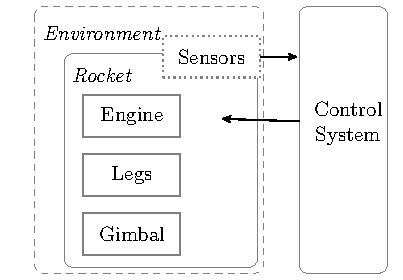
\includegraphics[width=\linewidth,origin=c]{overview.pdf}
  \caption{Interaction between system}
  \label{fig:overview}
\end{figure}

\subsection{Triple Modular Redundancy}

We aim at imitating a triple sensor system, where the control system receives three sensor values.
These values may at random be erroneous, and the control system takes the median of the received values.

\section{Controlling the Rocket}

We did two types of controllers.

\subsection{Bang-Bang}

Bang-bang control is a control technique used to reach some target.
It is called ``bang-bang'' because the controller simply says on or off.
There is no in-between.
One big con is that it most likely will overshoot its target multiple times because the system does not adjust according to its current location.

\subsection{Proportional–Integral–Derivative}

Proportional–Integral–Derivative (PID) control is a more sophisticated technique that combines the current information, past and future to compensate and reach the desired goal.
%
\[
  t = K_p e(t) + K_i \int_{t}^{0} e(\tau{}) d\tau{} + K_d \frac{de}{dt},
\]
%
where all $K$'s are non-negative values that should be adjusted by trial and error.
$e(t)$ computes the current error term from the desired target $t$.
$\tau$ denotes a constant for the slope.
$K_p, K_i, K_d$ denote the present, past and possible future values, respectively.

Actually we made it work with on PD.

\section{Simulation Results}

Figure \ref{fig:altitude} presents how the altitude of the rocket is very similar while comparing the Bang and PD controller.

\begin{figure}
  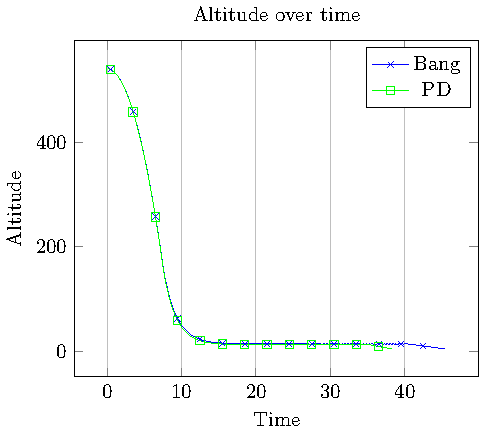
\includegraphics[width=\linewidth,origin=c]{altitude.pdf}
  \caption{Comparison altitude over time for Bang and PD.}
  \label{fig:altitude}
\end{figure}

Figure \ref{fig:tilt} shows how the rocket's tilt changes radically when gimbal is not compensating for the current position.
It actually gets worse.

\begin{figure}
  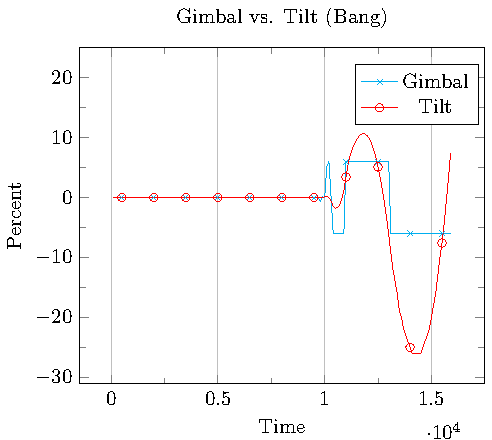
\includegraphics[width=\linewidth,origin=c]{tilt.pdf}
  \caption{Comparison of gimbal and tilt for Bang.}
  \label{fig:tilt}
\end{figure}

Figure \ref{fig:gimbal} shows that the PD control is much better at reaching the target and eventually stabilises elegantly.

\begin{figure}
  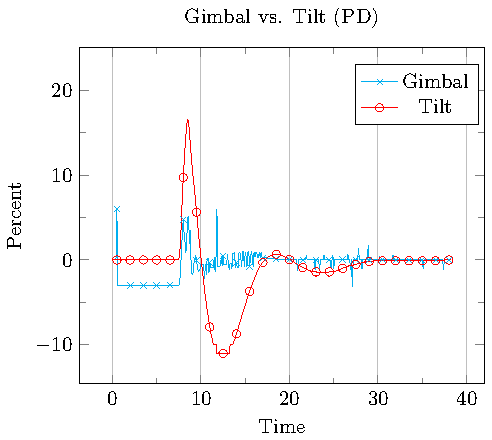
\includegraphics[width=\linewidth,origin=c]{gimbal.pdf}
  \caption{Comparison of gimbal and tilt for PD.}
  \label{fig:gimbal}
\end{figure}

Figure \ref{fig:thrust} illustrates how the thrust for Bang control looks very noisy because it turns on and off.
The PD control is more controlled and stabilises eventually and earlier than the Bang control does.

\begin{figure}
  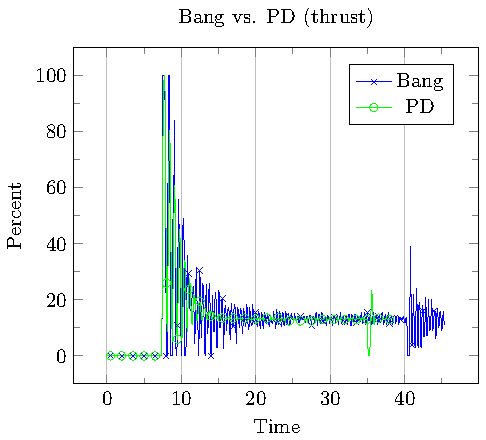
\includegraphics[width=\linewidth,origin=c]{thrust.pdf}
  \caption{Comparison thrust over time for Bang and PD.}
  \label{fig:thrust}
\end{figure}

\section{Conclusion}

Check out the awesome simulation video!

\end{dtupostercontent}

\end{document}
